\chapter{Experiments}
\label{ch:intro}

In order to evaluate our extension of ILP, the correlation and lattice, and the different interestingness measures, we
perform a series of experiments on Linked Data.

First, we test our proposed approach on LinkedMDB 

Firstly, we compare different measures by building same-sized correlation lattices on the $hasIncome(X,Y)$
relation from the USCensus, then searching for interesting rules with intervals for $Y$ inside the lattice itself as
described in Section~\ref{sec:searchRulesInCL}. The lattices are build by greedily choosing the top-k most interesting
nodes in each level according to the chosen measure, and pruning the rest so that all the lattices have the same
quantity of nodes.

Also, we measure the total time spent for the construction of each lattice as well as the number of interesting rules
found in it. As candidate categorical relations, we chose the 18 shown in Table~\ref{tab:uscensusRelations}. More
details about the categories can be found at the PUMS
Data
Dictionary\footnote{\url{http://www.census.gov/acs/www/Downloads/data_documentation/pums/DataDict/PUMSDataDict05_07.pdf}
}

\begin{table}[h!]
\begin{minipage}{\textwidth}
 \begin{center}
 \caption{Chosen categorical relations from USCensus}
  \begin{tabular}{l l c}
    \toprule
      Name	& Label				& Number of Categories \\
    \midrule
      sex	& Sex				&	2	\\
      st	& State				&	52\footnote{Including Puerto Rico and Washington D.C.}	\\
      racwht	& is White			&	2	\\
      racblk	& is Black			&	2	\\
      racasn	& is Asian			&	2	\\
      qtrbir	& Quarter of Birth		&	4	\\	
      nativity	& born In the US		&	2	\\
      mar	& Marital Status		&	5	\\
      lanp	& Language Spoken at Home	&	104	\\
      esr	& Employment Status		&	6	\\
      dphy	& Physical Difficulty		&	2	\\
      schl	& Educational Level		&	17	\\	
      occp	& Occupation			&	470	\\
      sch	& School Enrollment		&	3	\\
      rel	& Relationship			&	12	\\
      esp	& Employment Status of Parents	&	8	\\
      oc	& Own Child			&	2	\\
    \bottomrule
  \end{tabular}
 \label{tab:uscensusRelations}
 \end{center}
\end{minipage}
\end{table}




Since the USCensus data is completely joined on person entities, and all categorical relations have literals as
constants (usually integer numbers mapped to a set of) of entities 

***Roughly explaining the experiments I did so far, we want to evaluate whether the heuristics are good.
So we use US Census data to build a lattice (for income property) with the limitation of having up to $n$ nodes at each
level. So far I compared the KL-divergence*Support with support only as measures. For every level I sort the nodes by
the measure (nodes with multiple parents will have multiple KL-divergence, in this case I take the maximum one) and try
to join the nodes with highest measures first until $n$ nodes for the next level is reached. In other words, I greedily
build the a lattice with limited number of nodes per level.

After that, I try to extract rules with interesting ranges directly from the lattice and test them against a test
partition. Interesting rules are defined as in \refname{Interesting Rules} with support threshold of 25 examples and
accuracy threshold of 0.75. After that, I compare the number of interesting rules learned, the time taken to build the
lattice and the accuracy and accuracy gain compared to the base rule.

Accuracy and accuracy gain seem to depend exclusively on the accuracy threshold, so they are roughly the same for both
measures. Processing time is much smaller for the KL-divergence as it doesn't simply focus on huge relations and as
expected, it also presents a greater number of rules with interesting ranges (at least for smaller number of nodes per
level).

Hopefully I'll soon have results from applying the lattice in the core ILP. I managed to overcome some
implementation problems I had when creating the lattice in YAGO.

\begin{figure}
\caption{Lattices with 3 levels}
\centering
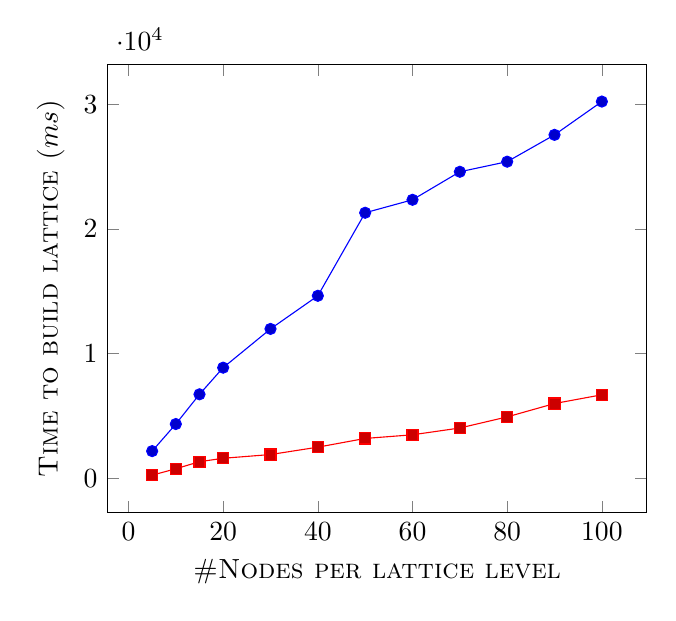
\begin{tikzpicture}[scale=1.0]
 \begin{axis}[
        xlabel=\textsc{\#Nodes per lattice level},
        ylabel=\textsc{Time to build lattice ($ms$)}
    ]
\addplot coordinates {(5,2165) (10,4337) (15,6723) (20,8860) (30,11969) (40,14626) (50,21288) (60,22329) (70,24577)
(80,25387) (90,27539) (100,30210)};
\addplot coordinates {(5, 235) (10,748) (15, 1317) (20, 1590) (30, 1890) (40, 2482) (50, 3182) (60, 3474) (70, 4020)
(80, 4911) (90,5982) (100,6684)};
\end{axis}
\end{tikzpicture}

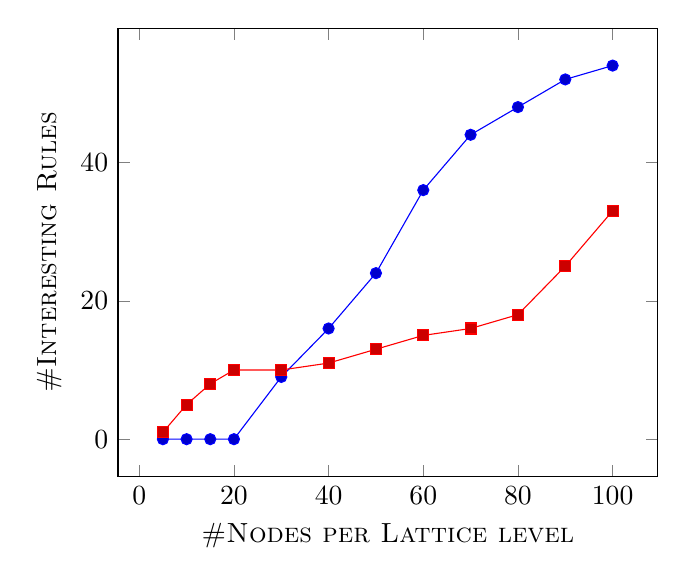
\begin{tikzpicture}[scale=1.0]
 \begin{axis}[
        xlabel=\textsc{\#Nodes per Lattice level},
        ylabel=\textsc{\#Interesting Rules}
    ]
\addplot coordinates {(5,0) (10,0) (15,0) (20, 0) (30, 9) (40,16) (50,24) (60,36) (70,44) (80,48) (90,52) (100,54)};
\addplot coordinates {(5,1) (10,5) (15,8) (20,10) (30,10) (40,11) (50,13) (60,15) (70,16) (80,18) (90,25) (100,33)};
\end{axis}
\end{tikzpicture}
\end{figure}

\begin{figure}
 \caption{Lattice with 4 levels}
 \centering
 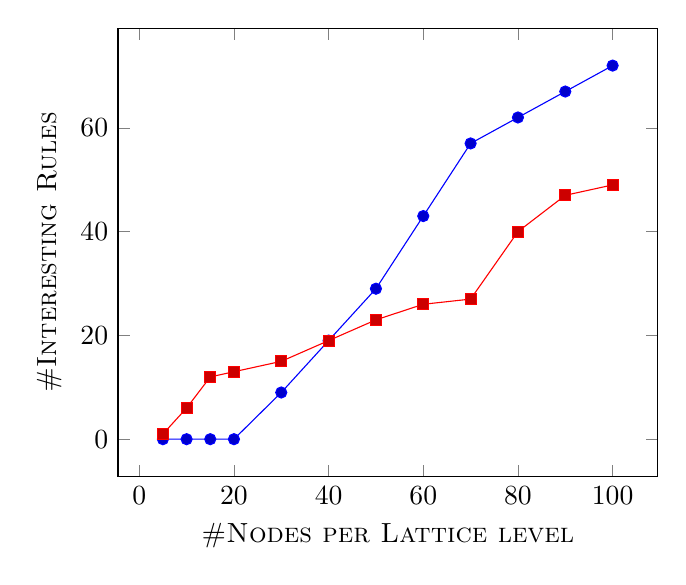
\begin{tikzpicture}[scale=1.0]
  \begin{axis}[
	  xlabel=\textsc{\#Nodes per Lattice level},
	  ylabel=\textsc{\#Interesting Rules}
      ]
  \addplot coordinates {(5,0) (10,0) (15, 0) (20, 0) (30, 9) (40,19) (50,29) (60,43) (70,57) (80,62) (90,67) (100,72)};
  %(110,75) (120,79) (130,84) (140,88) (150,94) (200,122) (250,159) (300,178) (350,200) (400,214) (450,231) (500,242)};
  \addplot coordinates {(5,1) (10,6) (15,12) (20,13) (30,15) (40,19) (50,23) (60,26) (70,27) (80,40) (90,47) (100,49)};
  %(110,) (120,) (130,) (140,) (150,) (200,) (250,) (300,) (350,) (400,) (450,) (500,)};
  \end{axis}
  \end{tikzpicture}
  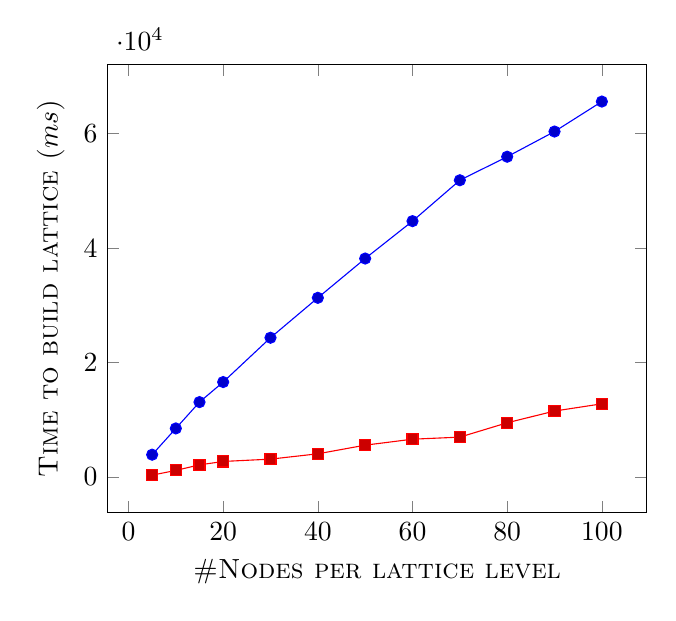
\begin{tikzpicture}[scale=1.0]
  \begin{axis}[
	  xlabel=\textsc{\#Nodes per lattice level},
	  ylabel=\textsc{Time to build lattice ($ms$)}
      ]
  \addplot coordinates {(5,3905) (10,8496) (15,13097) (20,16601) (30,24348) (40,31322) (50,38189) (60,44724) (70,51869)
  (80,55981) (90,60382) (100,65622)};
% (110,75) (120,79) (130,84) (140,88) (150,94) (200,122) (250,159) (300,178)  (350,200) (400,214) (450,231) (500,242)};
  \addplot coordinates {(5, 330) (10,1161) (15, 2128) (20, 2722) (30, 3130) (40, 4060) (50, 5571) (60, 6613) (70, 6976)
  (80, 9483) (90,11534) (100,12795)};
% (110,) (120,) (130,) (140,) (150,) (200,) (250,) (300,) (350,) (400,) (450,) (500,)};
  \end{axis}
  \end{tikzpicture}
\end{figure}

\begin{figure}
 \caption{Recall-Accuracy }
 \centering
 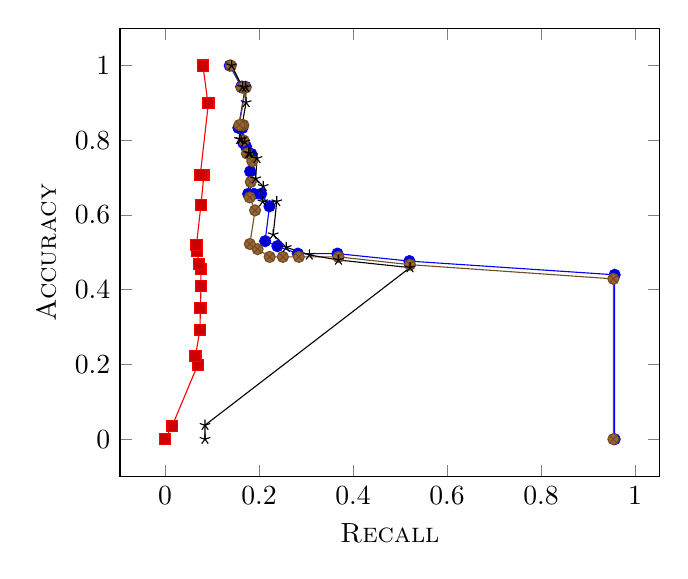
\begin{tikzpicture}[scale=1.0]
  \begin{axis}[
	  xlabel=\textsc{Recall},
	  ylabel=\textsc{Accuracy}
      ]
  \addplot coordinates {(0.9565217,0) (0.9565217,0.44) (0.52,0.4766667) (0.3669951,0.4966667) (0.2827325 ,
0.4966667) (0.2391975,0.5166667) (0.2131367,0.53) (0.2223543,0.6233333) (0.2045691,0.6566667) (0.1894231 ,
0.6566667) (0.1769991,0.6566667) (0.1812816,0.7166666) (0.1839358,0.7633333) (0.1724138,0.7833334) (0.1665500 ,
0.7933334) (0.1649076,0.8333333) (0.1612903,0.8333333) (0.15625,0.8333333) (0.1711004,0.9433333) (0.1644393 ,
0.9433333) (0.1623637,0.9433333) (0.1379310,1)};
  \addplot coordinates {(0,0) (0,0) (0,0) (0,0) (0.01530612,0.03508772) (0.0698152,0.1988304) (0.06495727 ,
0.2222222) (0.07440476,0.2923977) (0.07556675,0.3508772) (0.07667032,0.4093567) (0.07617188,0.4561403)
(0.07181329,0.4678363) (0.06907631,0.502924) (0.06711916,0.5204678) (0.0764832,0.625731) (0.0829904,0.7076023)
(0.0810992,0.7076023) (0.07846952,0.7076023) (0.07520199,0.7076023) (0.09260373,0.9005848) (0.09139466 ,
0.9005848) (0.08077468,1)};
  \addplot coordinates { (0.9538462,0) (0.9538462,0.4290657) (0.5212355,0.467128) (0.3691100,0.4878893)
(0.2848485,0.4878893) (0.2508897,0.4878893) (0.2227488,0.4878893) (0.1970509,0.5086505) (0.180622,0.5224913)
(0.1917660,0.6124567) (0.1803279,0.6470588) (0.1825688,0.6885813) (0.1858254,0.7439446) (0.1744278,0.7647059)
(0.1676343,0.799308) (0.1667810,0.8408305) (0.1631968,0.8408305) (0.1583062,0.8408305) (0.1718256,0.9411765)
(0.1654501,0.9411765) (0.1634615,0.9411765) (0.1401552,1)};
  \addplot coordinates {(0.08527132,0) (0.08527132,0.03741496) (0.5212355,0.4591837) (0.3691100,0.4795918)
(0.3072034,0.4931973)
(0.2581197,0.5136054) (0.2303290,0.547619) (0.2379135,0.6360544) (0.2080089,0.6360544) (0.2090336,0.6768708)
(0.193032,0.6972789) (0.1957484,0.7517007) (0.1810137,0.7653061) (0.1781473,0.7653061) (0.1696882,0.7959183)
(0.1621993,0.8027211) (0.1587088,0.8027211) (0.1726384,0.9013606) (0.1716233,0.9421769) (0.1653731,0.9421769)
(0.1418234,1)};
  \end{axis}
  \end{tikzpicture}
\end{figure}

\begin{figure}
 \caption{Runtime-LearnedRules}
 \centering
 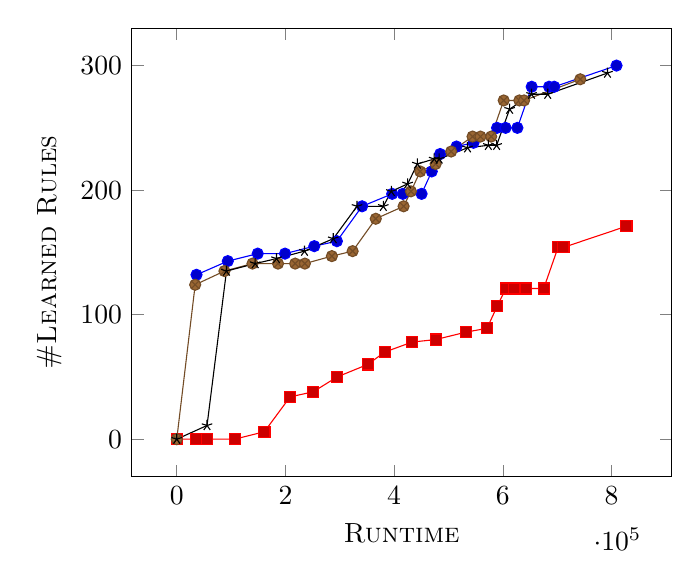
\begin{tikzpicture}[scale=1.0]
  \begin{axis}[
	  xlabel=\textsc{Runtime},
	  ylabel=\textsc{\#Learned Rules}
      ]
  \addplot coordinates { (36343,132) (93944,143) (148944,149) (199223,149) (253104,155) (294678,159) (341024,187)
(396459,197) (416000,197) (450504,197) (469231,215) (484591,229) (514785,235) (546069,238) (589417,250) (605128,250)
(626821,250) (653140,283) (685085,283) (694687,283) (809238,300)};
  \addplot coordinates {(0,0) (35466,0) (55421,0) (106586,0) (161302,6) (208629,34) (250863,38) (295212,50) (351300,60)
(382899,70) (433423,78) (476677,80) (532442,86) (570818,89) (589925,107) (605518,121) (621333,121) (643190,121)
(675208,121) (701631,154) (711515,154) (827520,171)};
  \addplot coordinates {(0,0) (33892,124) (87747,135) (139353,141) (186294,141) (217893,141) (235750,141) (285443,147)
(323626,151) (366197,177) (417438,187) (430932,199) (447970,215) (476371,221) (504948,231) (544307,243) (558897,243)
(578569,243) (601647,272) (630384,272) (639120,272) (742514,289)};
  \addplot coordinates {(0,0) (55709,11) (91488,135) (144319,141) (183567,145) (235053,151) (288040,161) (331747,187)
(380080,187) (394814,199)
(424827,205) (442860,221) (473691,225) (482918,225) (535099,234) (573386,236) (588600,236) (612505,265) (652833,277)
(682636,277) (792557,294)};
  \end{axis}
  \end{tikzpicture}
\end{figure}


\subsection{Example of Rules Learned}

We selected a couple of interesting rules learned with our approach in order to illustrate the kind of results we
obtain. On LinkedMDB, for example, we learned that films in English with Canadian director, and low budget are
significantly more likely to be also Canadian than those with higher budget. The base rule shown below has
confidence $0.36$:

$country(X,canada)$ :- $director(X,Z),bornIn(Z,canada),language(X,english),budget(X,Y)$

When we refine this rule, we find an interval with confidence $0.83$:

$country(X,canada)$ :- $director(X,Z),bornIn(Z,canada),language(X,english),budget(X,Y),Y\leq 80000$

Another interesting example reveals that films written by a spouse of Fritz Lang (in this case, Thea von
Harbou, who was an actress, writer, and director), and which have long runtime are more likely to have been directed by
Fritz Lang than those with shorter runtime. The base rule has confidence $0.6$:

$director(X,fritzLang)$ :- $writer(A,D),spouse(D,fritzLang),runtime(X,Y)$

And the refined rule has confidence $0.82$:

$director(X,fritzLang)$ :- $writer(A,D),spouse(D,fritzLang),runtime(X,Y),Y\geq 6800s$

Other examples of interesting rules learned are shown in Table~\ref{tab:mdbRuleExamples}.

\begin{table}[h!]
\begin{minipage}{\textwidth}
 \begin{center}
 \caption{Interesting rules with numerical intervals}
  \begin{tabular}{ >{\emph}r >{\raggedright}p{7cm} | c | c }
    \toprule
      & Refined Rule				& Conf 	& Gain \\
    \midrule
      director(X,fritzLang) :-&writer(X,Z), spouse(Z,fritzLang), runtime(X,Y), Y$\geq 6800s$ & 
      0.82	& 0.37 \\
      writer(X,sylvesterStallone) :-&starring(X,sylvesterStallone), subject(X,englishLanguageFilms),
      budget(X,Y), Y$\in [6M,31M]$ &
      0.89	& 0.48 \\
      producer(X,clintEastwood) :-&director(X,clintEastwood), starring(X,clintEastwood),
      subject(X,englishLanguageFilms), budget(X,Y), Y$\geq 13M$ &
      1.00	& 0.73 \\
      starring(X,clintEastwood) :- &budget(X,Y), director(X,clintEastwood), starring(A,clintEastwood), 
      subject(A,englishLanguageFilms), Y$\in [930K,25M]$&
      0.82	& 0.56 \\
      starring(X,Z) :-&writer(X,Z), country(X,uk), distributor(X,bbc),r untime(X,Y), Y$\leq 4080s$ &
      0.9	& 0.53 \\

    \bottomrule
  \end{tabular}
 \label{tab:mdbRuleExamples}
 \end{center}
\end{minipage}
\end{table}


On the

\begin{table}[h!]
\begin{minipage}{\textwidth}
 \begin{center}
 \caption{Interesting rules with numerical intervals}
  \begin{tabular}{ >{\textit}r >{\raggedright}p{7cm} | c | c }
    \toprule
      & Refined Rule				& Conf 	& Gain \\
    \midrule
      director(X,fritzLang) :-&writer(X,Z), spouse(Z,fritzLang), runtime(X,Y), Y$\geq 6800s$ & 
      0.82	& 0.37 \\
      writer(X,sylvesterStallone) :-&starring(X,sylvesterStallone), subject(X,englishLanguageFilms),
      budget(X,Y), Y$\in [6M,31M]$ &
      0.89	& 0.48 \\
      producer(X,clintEastwood) :-&director(X,clintEastwood), starring(X,clintEastwood),
      subject(X,englishLanguageFilms), budget(X,Y), Y$\geq 13M$ &
      1.00	& 0.73 \\
      starring(X,clintEastwood) :- &budget(X,Y), director(X,clintEastwood), starring(A,clintEastwood), 
      subject(A,englishLanguageFilms), Y$\in [930K,25M]$&
      0.82	& 0.56 \\
      starring(X,Z) :-&writer(X,Z), country(X,uk), distributor(X,bbc),r untime(X,Y), Y$\leq 4080s$ &
      0.9	& 0.53 \\

    \bottomrule
  \end{tabular}
 \label{tab:ruleExamples}
 \end{center}
\end{minipage}
\end{table}



\begin{figure}
 \caption{Recall-Accuracy }
 \centering
 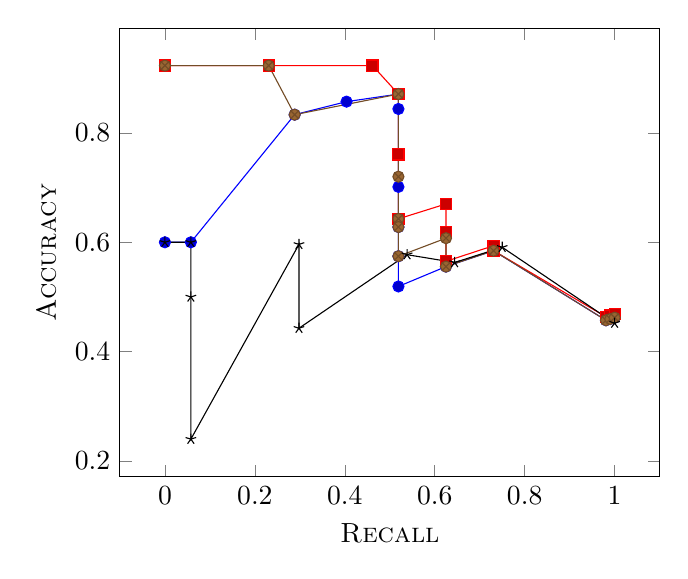
\begin{tikzpicture}[scale=1.0]
  \begin{axis}[
	  xlabel=\textsc{Recall},
	  ylabel=\textsc{Accuracy}
      ]
  \addplot coordinates {(0,0.6) (0.05769231,0.6) (0.2884615,0.8333333) (0.4038461,0.8571429) (0.5192308
, 0.8709678) (0.5192308,0.84375) (0.5192308,0.7012987) (0.5192308,0.627907) (0.5192308,0.5744681) (
0.5192308,0.5192308) (0.625,0.5555556) (0.7307692,0.5846154) (0.9807692,0.4573991) (0.9903846 ,
0.4598214) (1,0.4622222)};
  \addplot coordinates {(0,0.9230769) (0.2307692,0.9230769) (0.4615385,0.9230769) (0.5192308,0.8709678)
(0.5192308,0.7605634) (0.5192308,0.6428571) (0.625,0.6701031) (0.625,0.6190476) (0.625,0.5652174) (
0.7307692,0.59375) (0.7307692,0.5846154) (0.9807692,0.4636364) (0.9903846,0.4660633) (1,0.4684685)};
  \addplot coordinates { (0,0.9230769) (0.2307692,0.9230769) (0.2884615,0.8333333) (0.5192308,0.8709678)
(0.5192308,0.72) (0.5192308,0.6428571) (0.5192308,0.627907) (0.5192308,0.5744681) (0.625,0.6074766)
(0.625,0.5555556) (0.7307692,0.5846154) (0.9807692,0.4573991) (0.9903846,0.4598214) (1,0.4622222)};
  \addplot coordinates {(0,0.6) (0.05769231,0.6) (0.05769231,0.5) (0.05769231,0.24) (0.2980769 ,
0.5961539) (0.2980769,0.4428571) (0.5384616,0.5773196) (0.6442308,0.5630252) (0.75,0.5909091) (1 ,
0.4521739)};
  \end{axis}
  \end{tikzpicture}
\end{figure}

\begin{figure}
 \caption{Runtime-LearnedRules}
 \centering
 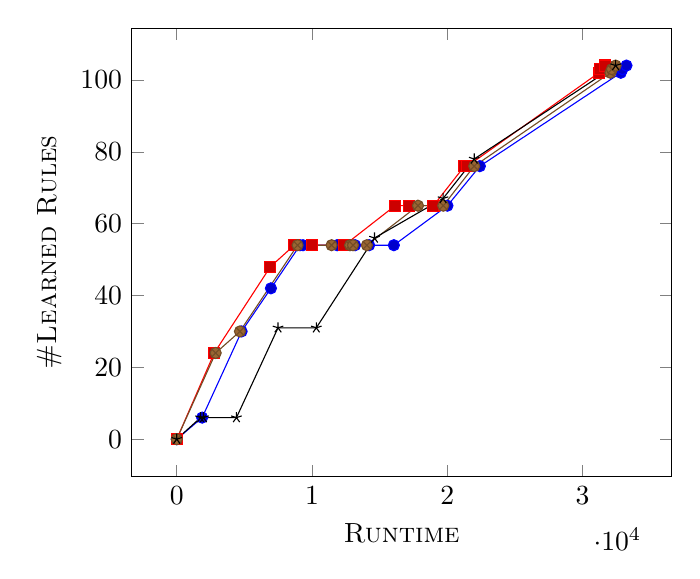
\begin{tikzpicture}[scale=1.0]
  \begin{axis}[
	  xlabel=\textsc{Runtime},
	  ylabel=\textsc{\#Learned Rules}
      ]
  \addplot coordinates {(0,0) (1877,6) (4795,30) (6962,42) (9116,54) (9337,54) (11852,54) (
13187,54) (14225,54) (16052,54) (20014,65) (22411,76) (32833,102) (32949,103) (33251,104
)};
  \addplot coordinates {(0,0) (2772,24) (6923,48) (8690,54) (9977,54) (12400,54) (16145,65)
(17187,65) (18979,65) (21270,76) (21483,76) (31215,102) (31324,103) (31637,104)};
  \addplot coordinates {(0,0) (2877,24) (4672,30) (8934,54) (11447,54) (12813,54) (13033,54)
(14057,54) (17836,65) (19703,65) (21991,76) (32064,102) (32173,103) (32449,104)};
  \addplot coordinates { (0,0) (1762,6) (1976,6) (4413,6) (7488,31) (10319,31) (14620,56) (
19691,67) (21995,78) (32452,104)};
  \end{axis}
  \end{tikzpicture}
\end{figure}


